%%
%% Joint Seed Selection and Discounting for Revenue Maximization
%% in Social Networks via Deep Reinforcement Learning
%%
%% Target venue: WSDM 2028 (ACM sigconf)
%%
%% ── COMPILE ──────────────────────────────────────────────────────────────────
%%   pdflatex main.tex && bibtex main && pdflatex main.tex && pdflatex main.tex
%%   (Overleaf: Menu → Compiler → pdfLaTeX)
%%
%% ── BLIND/CAMERA SWITCH ──────────────────────────────────────────────────────
%%   Blind submission : \documentclass[sigconf,review,anonymous]{acmart}  ← THIS
%%   Camera-ready    : \documentclass[sigconf]{acmart}  (uncomment real authors)
%% ─────────────────────────────────────────────────────────────────────────────

\documentclass[sigconf,review,anonymous]{acmart}

%% ── Math ─────────────────────────────────────────────────────────────────────
\usepackage{amsmath, amssymb, amsthm}

%% ── Tables ───────────────────────────────────────────────────────────────────
\usepackage{booktabs}
\usepackage{multirow}
\usepackage{tabularx}

%% ── Algorithms ───────────────────────────────────────────────────────────────
\usepackage{algorithm}
\usepackage{algpseudocode}

%% ── Figures ──────────────────────────────────────────────────────────────────
\usepackage{subcaption}
\graphicspath{{figures/}}              % all figures mirrored to paper/figures/

%% ── Float / spacing control ──────────────────────────────────────────────────
\usepackage{placeins}
\usepackage{float}
\setlength{\textfloatsep}{8pt plus 2pt minus 2pt}
\setlength{\floatsep}{6pt plus 2pt minus 2pt}
\setlength{\intextsep}{8pt plus 2pt minus 2pt}
\setlength{\abovecaptionskip}{4pt}
\setlength{\belowcaptionskip}{2pt}

%% ── Enumeration ──────────────────────────────────────────────────────────────
\usepackage{enumitem}

%% ── Hyperlinks (loaded last to avoid clashes) ────────────────────────────────
%% acmart loads hyperref internally; add options via:
%% \hypersetup{hidelinks}

%% ── Theorem environments ─────────────────────────────────────────────────────
\newtheorem{definition}{Definition}
\newtheorem{problem}{Problem}
\newtheorem{proposition}{Proposition}

%% ── Convenience math macros ──────────────────────────────────────────────────
\DeclareMathOperator*{\argmax}{arg\,max}
\DeclareMathOperator*{\argmin}{arg\,min}
\newcommand{\R}{\mathbb{R}}
\newcommand{\calG}{\mathcal{G}}
\newcommand{\calV}{\mathcal{V}}
\newcommand{\calE}{\mathcal{E}}
\newcommand{\calS}{\mathcal{S}}
\newcommand{\St}{S_t}               % seed set at step t
\newcommand{\val}{v}                % valuation function

%% ── ACM metadata (suppressed for blind review) ───────────────────────────────
\settopmatter{printacmref=false}
\renewcommand\footnotetextcopyrightpermission[1]{}
\setcopyright{none}
%% Fill in real values for camera-ready:
\acmConference[WSDM '28]{The 21st ACM International Conference on Web Search
  and Data Mining}{February 2028}{TBD}
\acmYear{2028}
\copyrightyear{2028}
\acmISBN{}
\acmDOI{}
\acmPrice{}

%% ── Title ────────────────────────────────────────────────────────────────────
\title{Joint Seed Selection and Discounting for Revenue Maximization\\
       in Social Networks via Deep Reinforcement Learning}

%% ── Authors (comment out entire block for blind submission;
%%    anonymous class option already removes them, but keep consistent) ─────────
%% Camera-ready: uncomment and fill in real affiliations
%
% \author{Fatemeh Seyedin}
% \affiliation{\institution{Leibniz University Hannover}\country{Germany}}
%
% \author{Adrian Weller}
% \affiliation{\institution{University of Cambridge}\country{United Kingdom}}
%
% \author{Mahmoudreza Babaei}
% \affiliation{\institution{GISMA University of Applied Sciences}\country{Germany}}
%
% \renewcommand{\shortauthors}{Seyedin et al.}

%% ═══════════════════════════════════════════════════════════════════════════
\begin{document}

%% ── Abstract (must appear before \maketitle in acmart) ───────────────────────
\begin{abstract}
% paper/sections/abstract.tex
% Target: ~170 words (WSDM 2028 double-blind submission)
% Style: CrossWalk/Adv.GE house style — context→gap→"Here,we"→numbers→framing→caveat
%
% NUMBER SOURCES (every number below has a cited JSON):
%   462.6  % SOURCE: CLAUDE.md §Session State; results/logs/comparison_20260623_131609.json
%   460.0  % SOURCE: CLAUDE.md §Session State; results/logs/comparison_20260623_131609.json
%   p<0.0001, 20/20  % SOURCE: CLAUDE.md §Session State
%   +8.6%  % SOURCE: results/logs/paper_gen_updated.json (FF n=2000, LSTM vs Greedy-Discount)
%   +40.5% % SOURCE: results/logs/paper_gen_updated.json (Rice-FB n=443, LSTM vs Greedy-Discount)
%   99.8   % SOURCE: results/logs/dp_v3_full_curve_merged.json (ff_n1000, k=3, v3/composite)
%   23.6   % SOURCE: results/logs/dp_upgrade_eval.json (k=3, Greedy+Budget: 23.62)
%   448    % SOURCE: results/logs/dp_v3_full_curve_merged.json (ff_n1000, k=40, v2: 448.0)
%   449    % SOURCE: results/logs/dp_upgrade_eval.json (k=40, Greedy+Budget: 448.66≈449)
%   305.6  % SOURCE: results/logs/unified_sweep.json (k=1, unified learned policy: 305.572)
%   7.4    % SOURCE: results/logs/dp_upgrade_eval.json (k=1, Greedy+Budget: 7.39≈7.4)

Revenue maximization via targeted discounting in social networks — offering personalized
prices to influential buyers so that peer-to-peer diffusion amplifies total sales —
has relied on two hand-crafted, decoupled steps: greedy seed selection followed by a
degree-rule pricing heuristic~\citep{babaei2013revenue}.
The coupling between \emph{who} to target and \emph{what price} to offer is ignored.
Here, we introduce the first end-to-end learning approach: a GNN--LSTM policy that
jointly selects seeds and sets personalized discounts via imitation learning and
REINFORCE.
%
Trained on graphs with $n \le 440$ nodes, the model achieves
$462.6$ %SOURCE: comparison_20260623_131609.json
revenue on Forest-Fire $n{=}1000$ versus $460.0$ for the best hand-crafted baseline
($p{<}0.0001$, $20/20$ seeds),
%SOURCE: CLAUDE.md §Session State
and transfers zero-shot to $n{=}2000$ ($+8.6\%$) %SOURCE: paper_gen_updated.json
and Rice-Facebook ($+40.5\%$). %SOURCE: paper_gen_updated.json
%
We further introduce a budget-constrained formulation in which a production cost is
deducted per offer from replenishable finite capital, casting selection as a
sequential knapsack with network externalities.
A calibrated dynamic-programming baseline dominates classical methods where the
budget binds
($99.8$ vs.\ $23.6$ at $k{=}3$) %SOURCE: dp_v3_full_curve_merged.json / dp_upgrade_eval.json
and matches greedy at large~$k$ ($448$ vs.\ $449$); %SOURCE: same
our learned policy reaches $305.6$ vs.\ $7.4$ at $k{=}1$ ($41{\times}$). %SOURCE: unified_sweep.json / dp_upgrade_eval.json
One honest finding: calibrated DP leads the learned policy at mid-$k$ on the
dense Rice-Facebook graph.

\end{abstract}

\maketitle

%% ── §1 Introduction ──────────────────────────────────────────────────────────
% paper/sections/introduction.tex
% Target: 0.9–1.1 pages (sigconf two-column ≈ 700–900 words body text)
% Style: WSDM framing — network economics first, learning as instrument.
%        Structure: P1 viral marketing+Babaei | P2 deep-IM gap (1 sentence) |
%                   P3 our approach | P4 budget realism | P5 C1–C4 bullets | P6 roadmap
% Every number has a %SOURCE comment. Phrases follow style_notes.md.
%
% ANONYMIZATION: cite WSDM 2027 prior work as \cite{anon_wsdm27}.
%
% NUMBER SOURCES:
%   462.6 / 460.0   % SOURCE: CLAUDE.md; results/logs/comparison_20260623_131609.json
%   p<0.0001 20/20  % SOURCE: CLAUDE.md §Session State
%   +8.6% n=2000    % SOURCE: results/logs/paper_gen_updated.json (FF n=2000)
%   +40.5% Rice-FB  % SOURCE: results/logs/paper_gen_updated.json (Rice-FB n=443)
%   99.8 / 23.6 k=3 % SOURCE: dp_v3_full_curve_merged.json / dp_upgrade_eval.json
%   305.6 / 7.4 k=1 % SOURCE: unified_sweep.json / dp_upgrade_eval.json

\section{Introduction}
\label{sec:intro}

% ── P1: Viral marketing + discounting + Babaei ────────────────────────────────
A firm selling a product through a social network faces a classical tension:
deep discounts convert hesitant buyers and trigger peer-to-peer
diffusion,  but they erode margin on every unit sold.
\citet{babaei2013revenue} formalized this trade-off as a
\emph{revenue maximization via discounting} problem: the seller sequentially
targets a set of buyers and offers each a personalized price, exploiting the
fact that a buyer's willingness-to-pay rises as more of her social contacts
have already purchased.
Their framework showed that calibrated discounts strictly dominate the
free-seeding paradigm of classical influence maximization~\citep{kempe2003maximizing}
in terms of total revenue.
The practical limitation is that they rely on two independent, hand-crafted
steps — greedy seed selection by degree centrality, then discount assignment via a
simple degree rule — designed separately and applied in sequence.
The coupling between \emph{which} buyer to target next and
\emph{what price} to offer is never exploited.

% ── P2: Deep IM gap (one sentence) ───────────────────────────────────────────
Deep reinforcement learning for influence maximization — notably
S2V-DQN~\citep{dai2017learning} and ToupleGDD~\citep{touplegdd} — achieves
strong results on the seed-selection subproblem but optimizes
\emph{diffusion reach}, not revenue, and assumes zero production cost and no pricing
decisions.

% ── P3: Our approach ─────────────────────────────────────────────────────────
Here, we close both gaps.
We extend the graph RL framework of our prior work~\citep{anon_wsdm27} to the
joint seed-and-pricing problem.
At each decision step a two-layer GraphSAGE encoder produces node embeddings
that capture both structural centrality and the current influence state of
every buyer.
An LSTM then compresses the full episode history — past offers, accept/reject
outcomes, running revenue — into a context vector that is concatenated with
the per-node embedding before scoring.
A~joint policy head then selects the next buyer (discrete) and outputs a
personalized discount $d_t \in [0,1]$ (continuous), trained first by imitation
of the \citet{babaei2013revenue} greedy expert and then refined by REINFORCE.
Trained only on Forest-Fire graphs with $n \le 440$ nodes, the model achieves
$462.6$ %SOURCE: CLAUDE.md; comparison_20260623_131609.json
revenue on the standard $n{=}1000$ test graph versus $460.0$ for the best
hand-crafted baseline ($p{<}0.0001$, %SOURCE: CLAUDE.md §Session State
$20/20$ seeds).
Zero-shot generalization: $+8.6\%$ at $n{=}2000$ %SOURCE: paper_gen_updated.json
and $+40.5\%$ on Rice-Facebook. %SOURCE: paper_gen_updated.json

% ── P4: Realism gap → budget formulation ─────────────────────────────────────
A second limitation of all prior work — including the unconstrained model
above — is the assumption of infinite capital: the firm can approach any buyer
at any cost.
In practice, a seller starts with finite budget $B_0 = k \cdot c$ and incurs a
unit production cost $c$ for \emph{every} offer, whether or not the buyer
accepts; successful sales replenish the budget.
This transforms seed selection into a \emph{sequential knapsack with network
externalities}: the policy must reason jointly about which buyers to skip,
in what order to approach them, and what price to offer, all under a live
cash-flow constraint.
We formalize this budget-constrained variant, introduce a
\emph{calibrated dynamic-programming} (Cal-DP) baseline that adapts classical
DP to replenishable-capital settings, and train a budget-aware learned policy
via imitation on Cal-DP trajectories followed by REINFORCE.

% ── P5: Contribution bullets C1–C4 ───────────────────────────────────────────
\smallskip
\noindent\textbf{Contributions.}
\begin{enumerate}[label=\textbf{C\arabic*.}, leftmargin=*, topsep=2pt,
                  itemsep=1pt, parsep=0pt]

  \item \textbf{Joint learning for revenue maximization.}
    We introduce the first end-to-end model for joint seed selection and
    personalized pricing in social networks.
    On Forest-Fire $n{=}1000$, the GNN+LSTM policy achieves
    $462.6$ %SOURCE: CLAUDE.md; comparison_20260623_131609.json
    vs.\ $460.0$ for the Babaei greedy baseline
    ($p{<}0.0001$, $20/20$ seeds). %SOURCE: CLAUDE.md §Session State

  \item \textbf{Zero-shot size and network generalization.}
    Trained on $n \le 440$, the model transfers without retraining to
    $n{=}2000$ ($+8.6\%$) %SOURCE: paper_gen_updated.json
    and to the real Rice-Facebook graph ($+40.5\%$), %SOURCE: paper_gen_updated.json
    demonstrating that the GNN+LSTM inductive bias learns
    topology-agnostic pricing strategies.

  \item \textbf{Budget-constrained formulation.}
    We formalize revenue maximization under replenishable finite capital as a
    sequential knapsack with network externalities, a practically
    relevant variant absent from prior work.

  \item \textbf{Calibrated DP + learned policy for the budget regime.}
    Our Cal-DP baseline achieves $99.8$ vs.\ $23.6$ for classical Greedy+Budget
    at $k{=}3$ ($4.2{\times}$); %SOURCE: dp_v3_full_curve_merged.json / dp_upgrade_eval.json
    the learned policy reaches $305.6$ vs.\ $7.4$ at $k{=}1$ ($41{\times}$). %SOURCE: unified_sweep.json / dp_upgrade_eval.json
    One honest finding: Cal-DP leads the learned policy at mid-$k$ on the
    dense Rice-Facebook graph — a result we report transparently as a
    regime-aware conclusion.

\end{enumerate}

% ── P6: Roadmap ───────────────────────────────────────────────────────────────
\smallskip
\noindent\textbf{Paper organization.}
\S\ref{sec:related} surveys related work.
\S\ref{sec:problem} formalizes unconstrained (\S\ref{sec:babaei}) and
budget-constrained (\S\ref{sec:budget}) revenue maximization.
\S\ref{sec:method} describes the GNN+LSTM model, training procedure, and
Cal-DP baseline.
\S\ref{sec:experiments} reports experimental results and the regime map.
\S\ref{sec:conclusion} concludes with limitations and future directions.


%% ── §2 Related Work ──────────────────────────────────────────────────────────
% paper/sections/related_work.tex
% Style: [Author et al., year] showed/proposed... 1-2 sentences each.
%        Gap introduced by "However," or "Yet,".

\section{Related Work}
\label{sec:related}

Revenue maximization in social networks builds on three lines of research:
influence maximization, mechanism design for network markets, and deep RL on graphs.

\paragraph{Influence maximization.}
\citet{kempe2003maximizing} formulated seed-set selection under the Independent
Cascade and Linear Threshold models, proving a $(1 - 1/e)$-approximation via
greedy hill climbing.
Subsequent work scaled this to large graphs through lazy evaluations, sketching,
and diffusion simulations~\citep{goyal2011celf++,tang2014influence,tang2015influence}.
\citet{dai2017learning} introduced S2V-DQN, where a structure2vec GNN produces
node embeddings and a DQN selects seeds; this line was extended to
ToupleGDD~\citep{touplegdd}, which uses graph attention and policy
gradients to achieve state-of-the-art spread on large networks.
Fair variants of influence maximization~\citep{fish2019gaps,tsang2019group}
restrict seed selection to satisfy demographic constraints;
\citet{khajehnejad2022crosswalk} reweight random-walk probabilities to equalize
cross-group diffusion.
However, all of these methods maximize \emph{spread}, not \emph{revenue}, and
assume zero production cost and no pricing structure.

\paragraph{Revenue maximization in networks.}
\citet{babaei2013revenue} showed that a seller can collect strictly more revenue by
offering personalized discounts rather than giving items free, because a buyer's
willingness-to-pay increases as more of her contacts purchase.
Their algorithm selects seeds greedily by degree and assigns prices via a hand-crafted
degree rule (the $\mu$-discount), keeping selection and pricing independent.
Subsequent work by \citet{singer2012win} and \citet{hartline2008optimal} studied
pricing in cascade models under different information assumptions, but focused on
optimal single-item auctions rather than sequential joint policies.
\citet{kempe2014maximizing} extended the revenue framework to general buyer
valuations, but again with decoupled seed selection and pricing.
We are the first to learn a joint policy end-to-end.

\paragraph{Graph neural networks for combinatorial optimization.}
\citet{khalil2017learning} used GNNs with policy gradients to solve graph
combinatorial problems such as Minimum Vertex Cover and Traveling Salesman.
\citet{ding2020erdos} combined GNNs with REINFORCE for the Maximum Cut problem.
Our work applies the same graph RL paradigm to the continuous-discrete joint action
$(v^*, d_t)$ of seed selection and personalized discount, with the additional
complexity of a valuation model that depends on the current seed set.

\paragraph{Sequential pricing and mechanism design.}
The posted-price mechanism literature~\citep{blumrosen2011posted,roughgarden2012supply}
studies how a seller sets prices for buyers arriving in sequence; revenue maximization
in this setting is studied under various buyer-arrival
models~\citep{chawla2010multi}.
Budget-limited influence maximization has been studied in the context of
advertising~\citep{nguyen2013budget,zhang2016maximizing}, but the budget there
limits the \emph{number} of seeds rather than the capital available for production.
Our formulation introduces a \emph{replenishable} budget that grows with accepted
sales, which to our knowledge has not appeared in prior work.

\paragraph{LSTM and Transformer for sequential optimization.}
Sequence models have been applied to combinatorial routing via pointer
networks~\citep{vinyals2015pointer} and to vehicle routing with
transformers~\citep{kool2019attention}.
\citet{chen2019learning} combined GNNs with LSTMs for local search on combinatorial
problems.
We use an LSTM to carry the episode history (past offers, acceptances, running revenue)
across steps, providing the policy with a compressed summary of how the network
responds to pricing, information that a stateless GNN cannot access.


%% ── §3 Problem Formulation ───────────────────────────────────────────────────
%%   §3.1 Babaei et al. (2013) — unconstrained revenue maximization
%%   §3.2 Budget-constrained formulation (our extension)
% paper/sections/problem_formulation.tex
% §3.1 Babaei (2013) unconstrained formulation
% §3.2 Our budget-constrained extension

\section{Problem Formulation}
\label{sec:problem}

We formalize two variants of the revenue maximization problem:
the unconstrained variant of \citet{babaei2013revenue} and our
budget-constrained extension.

\subsection{Unconstrained Revenue Maximization}
\label{sec:babaei}

Revenue maximization exploits the fact that social influence raises a buyer's
willingness-to-pay.

\begin{definition}[Influence Network]
Let $G = (\calV, \calE)$ be a directed weighted graph with edge weights
$w_{ij} \in [0,2]$ drawn independently from $\mathrm{Uniform}(0,2)$,
representing the influence strength of buyer $j$ on buyer $i$.
\end{definition}

\begin{definition}[Valuation]
Given seed set $\St \subseteq \calV$, the \emph{normalized influence} on buyer
$i$ is
\[
  x_i(\St) = \frac{\sum_{j \in \St \cup \{i\}} w_{ij}}{\sum_{k \in \calV} w_{ik}},
\]
and the \emph{valuation} (willingness-to-pay) of buyer $i$ is
$\val_i(\St) = f\!\left(2 x_i(\St)\right)$,
where $f$ is the Rayleigh CDF: $f(y) = (y/b^2)\exp(-y^2/2b^2)$, $b=1$.
The monotone variant clips $f$ to be non-decreasing (used for Forest-Fire graphs);
the non-monotone variant uses the raw Rayleigh PDF (used for Rice-Facebook).
\end{definition}

\begin{definition}[Offer and Acceptance]
At step $t$ the seller presents buyer $v^* \notin \St$ with price
$p_t = \val_{v^*}(\St) \cdot (1 - d_t)$, where $d_t \in [0,1]$ is the discount.
Buyer $v^*$ accepts if $p_t \le \val_{v^*}(\St)$
(equivalently, always accepts since $p_t \le \val_{v^*}(\St)$ by construction).
In practice we model stochastic acceptance: $v^*$ accepts with probability
$p_t / \val_{v^*}(\St) = 1 - d_t$ when the seller does not know the exact
weight realization and uses 200 Monte Carlo samples to estimate
$\hat{\val}_{v^*}(\St)$.
\end{definition}

Revenue from step $t$ is $r_t = p_t \cdot \mathbf{1}[\text{accepted}]$.
The seller's objective is:

\begin{problem}[Unconstrained Revenue Maximization]\label{prob:uncon}
Choose a sequence of buyers $v_1, \ldots, v_n$ and discounts $d_1, \ldots, d_n$
to maximize total revenue $R = \sum_{t=1}^{n} r_t$,
over all $n = |\calV|$ sequential offers.
\end{problem}

\noindent
The key difficulty is the \emph{joint coupling}: the revenue-optimal discount for
$v^*$ at step $t$ depends on the current influence $x_{v^*}(\St)$, which depends on
which buyers accepted in steps $1, \ldots, t-1$.
\citet{babaei2013revenue} ignore this coupling; we learn it end-to-end.

\subsection{Budget-Constrained Revenue Maximization}
\label{sec:budget}

Budget constraints transform seed selection into a sequential knapsack with
network externalities.

\begin{definition}[Production Cost and Capital]
The seller starts with capital $B_0 = k \cdot c$ for a given
\emph{initial target count} $k$ and unit production cost $c > 0$.
Each offer costs $c$ regardless of acceptance; successful sales replenish the
budget by the accepted price $p_t$.
The budget after step $t$ is:
\[
  B_{t} = B_{t-1} - c + r_t.
\]
\end{definition}

\begin{definition}[Bankruptcy]
The seller goes bankrupt at the first step $t$ for which $B_t < c$.
Once bankrupt, no further offers can be made.
\end{definition}

\begin{problem}[Budget-Constrained Revenue Maximization]\label{prob:budget}
Maximize total revenue $R = \sum_t r_t$ subject to solvency: $B_t \ge 0$ for all $t$.
\end{problem}

\noindent
Problem~\ref{prob:budget} strictly generalizes Problem~\ref{prob:uncon}:
as $c \to 0$ the constraint becomes vacuous.
With finite $c$, the policy must balance two competing effects.
\begin{itemize}[leftmargin=*,topsep=2pt,itemsep=0pt]
  \item \emph{Deep discounts} increase acceptance probability and revenue per step,
    replenishing the budget for future offers.
  \item \emph{Shallow discounts} (high prices) yield larger revenue per accepted
    buyer but risk rejection, draining the budget without replenishment.
\end{itemize}
Skipping low-value buyers (those unlikely to accept at a profitable price) becomes
a legitimate strategy to preserve budget for high-value opportunities later —
a decision that is NP-hard to optimize globally~\citep{papadimitriou1994complexity}.

\paragraph{Regime characterization.}
Let $k$ be the initial target count and $c = 0.3$ (our experimental setting).
The budget $B_0 = kc$ spans three qualitatively different regimes:
\begin{enumerate}[leftmargin=*,topsep=2pt,itemsep=0pt]
  \item \emph{Capital-binding} ($k \le 5$, $B_0 \le 1.5$):
    a single rejection can cause bankruptcy; skip decisions dominate.
  \item \emph{Transitional} ($6 \le k \le 15$, $1.8 \le B_0 \le 4.5$):
    skipping is beneficial but not mandatory; rich solution landscape.
  \item \emph{Budget-slack} ($k \ge 20$, $B_0 \ge 6.0$):
    capital rarely binds; the problem reduces approximately to the unconstrained
    variant.
\end{enumerate}
Our algorithms are evaluated across all three regimes (§\ref{sec:exp_budget}).


%% ── §4 Method ────────────────────────────────────────────────────────────────
%%   §4.1 GNN encoder + joint Beta heads
%%   §4.2 LSTM sequence model
%%   §4.3 Imitation → REINFORCE + mixed-expert training
%%   §4.4 Calibrated dynamic-programming baseline
% paper/sections/methodology.tex
% §4.1 GNN encoder + joint heads
% §4.2 LSTM sequence model
% §4.3 Training: imitation → REINFORCE + mixed expert
% §4.4 Calibrated DP baseline

\section{Method}
\label{sec:method}

Our model — Rev-GNN-LSTM — consists of a GraphSAGE encoder,
an LSTM episode-history module, and two joint output heads that simultaneously
select the next buyer and set a personalized discount.

\subsection{Node Feature Representation}
\label{sec:features}

Each node $i \in \calV$ at step $t$ is represented by a 21-dimensional feature vector
$\phi_i^{(t)} \in \R^{21}$ composed of three groups.

\emph{Static structural features} (dims 1–10, identical to~\citet{anon_wsdm27}):
degree rank, clustering coefficient, betweenness centrality, PageRank,
$k$-core number, eigenvector centrality, triangle count, closeness centrality,
eccentricity, and average neighbor degree.

\emph{Dynamic state features} (dims 11–16):
seed flag $\mathbf{1}[i \in \St]$, round ratio $t/n$,
fraction of $i$'s neighbors already in $\St$,
$\log(1 + \deg(i))$, clustering coefficient (repeated as diffusion signal),
and group flag (set to 0 for the revenue task).

\emph{Pricing-specific features} (dims 17–21, new):
normalized influence $x_i(\St)$,
estimated valuation $\hat{\val}_i(\St)$ from 200 Monte Carlo samples,
an offered-and-rejected flag,
steps-remaining ratio $(n - t)/n$,
and current budget ratio $B_t / B_0$ (dims 17–21; dim 21 is $0$ for the
unconstrained problem).

\subsection{GNN Encoder}
\label{sec:gnn}

A two-layer GraphSAGE~\citep{hamilton2017inductive} encoder with residual
connections and LayerNorm maps each node's feature vector to a 64-dimensional
embedding:
\begin{align}
  h_i^{(0)} &= \mathrm{ReLU}(\mathrm{LN}(W_{\mathrm{proj}}\,\phi_i^{(t)})),\\
  h_i^{(l)} &= \mathrm{ReLU}\!\left(\mathrm{LN}\!\left(h_i^{(l-1)}
    + W_{\mathrm{self}} h_i^{(l-1)}
    + W_{\mathrm{neigh}} \tfrac{1}{|\calN(i)|}\sum_{j\in\calN(i)} h_j^{(l-1)}
  \right)\!\right).
\end{align}
All weight matrices are shared across graphs and steps.

\subsection{LSTM Episode-History Module}
\label{sec:lstm}

A stateless GNN sees only the current step's graph embedding; it cannot reason
about pricing signals revealed by past offers, such as a network that
consistently rejects discounts below 40\%.
We address this with an LSTM over the episode trajectory.

At each step $t$, the LSTM receives a token
\[
  \tau_t = \bigl[\bar{h}^{(t)}\;\|\; d_{t-1}\;\|\; a_{t-1}\;\|\; r_{t-1}\bigr]
  \in \R^{67},
\]
where $\bar{h}^{(t)} = \frac{1}{|\calV|}\sum_i h_i^{(2)}$ is the mean-pooled
graph embedding, $d_{t-1}$ is the last discount offered, $a_{t-1} \in \{0,1\}$
is the acceptance indicator, and $r_{t-1}$ is the revenue collected.
The LSTM hidden state $c_t \in \R^{64}$ summarizes the full history.

\subsection{Joint Policy Heads}
\label{sec:heads}

For each unvisited node $i \notin \St$ the full context embedding is
\[
  z_i^{(t)} = \bigl[h_i^{(2)}\;\|\; c_t\bigr] \in \R^{128}.
\]
Two heads share this representation:

\emph{Scoring head}: $s_i = \mathrm{Linear}_{32\to1}(\mathrm{ReLU}(\mathrm{Linear}_{128\to32}(z_i^{(t)})))$.
The agent selects $v^* = \argmax_{i \notin \St} s_i$.

\emph{Pricing head}: a two-layer MLP that outputs the parameters
$(\alpha, \beta)$ of a Beta distribution over the discount $d_t \in [0,1]$:
\[
  (\alpha, \beta) = \mathrm{Softplus}\!\left(\mathrm{Linear}_{32\to2}(\mathrm{ReLU}(\mathrm{Linear}_{128\to32}(z_{v^*}^{(t)})))\right) + 1.
\]
During training the discount is sampled $d_t \sim \mathrm{Beta}(\alpha,\beta)$;
during evaluation we use the mean $d_t = \alpha/(\alpha+\beta)$.

\subsection{Training: Imitation then REINFORCE}
\label{sec:training}

Training proceeds in two phases, following the mixed-expert
schedule of~\citet{anon_wsdm27}.

\paragraph{Phase 1 — Imitation learning (300 epochs).}
We generate expert trajectories using the Greedy-Discount algorithm of
\citet{babaei2013revenue}.
For each expert trajectory we minimize a cross-entropy loss on the selection
head and a Beta-distribution negative log-likelihood on the pricing head.
Training graphs: 5 Forest-Fire graphs with $n \in \{200, 260, 320, 380, 440\}$,
drawn with $p=0.37$, $p_b=0.32$.
After Phase 1 the cross-entropy loss decreases from $4.96$ to $2.68$.

\paragraph{Phase 2 — REINFORCE (200 epochs).}
We fine-tune the full policy (selection $+$ pricing) with REINFORCE.
To stabilize training across the wide range of episode lengths and budget values,
we group episodes by budget size into five buckets
(corresponding to $k \in \{1\text{–}2, 3\text{–}5, 6\text{–}10, 11\text{–}20, 21\text{–}40\}$)
and maintain a per-bucket Welford running mean and standard deviation for
advantage normalization.
The entropy bonus coefficient is $\lambda_H = 0.01$ and the learning rate is
$5 \times 10^{-5}$.
The best checkpoint is selected by the maximum of the minimum per-bucket
mean reward.

A single policy trained across all budgets must reconcile opposing
strategies: capital-binding episodes reward conservative self-funding,
budget-slack episodes reward aggressive seeding.
To remove this compromise we additionally train a large-$k$ specialist on
$k \in [16, 40]$ only, warm-started from the unified model with the
identical recipe.
At deployment the checkpoint is selected by budget regime, mirroring the
per-$k$ composition of our Cal-DP baseline.
Both checkpoints are released.

\begin{figure}[t]
  \centering
  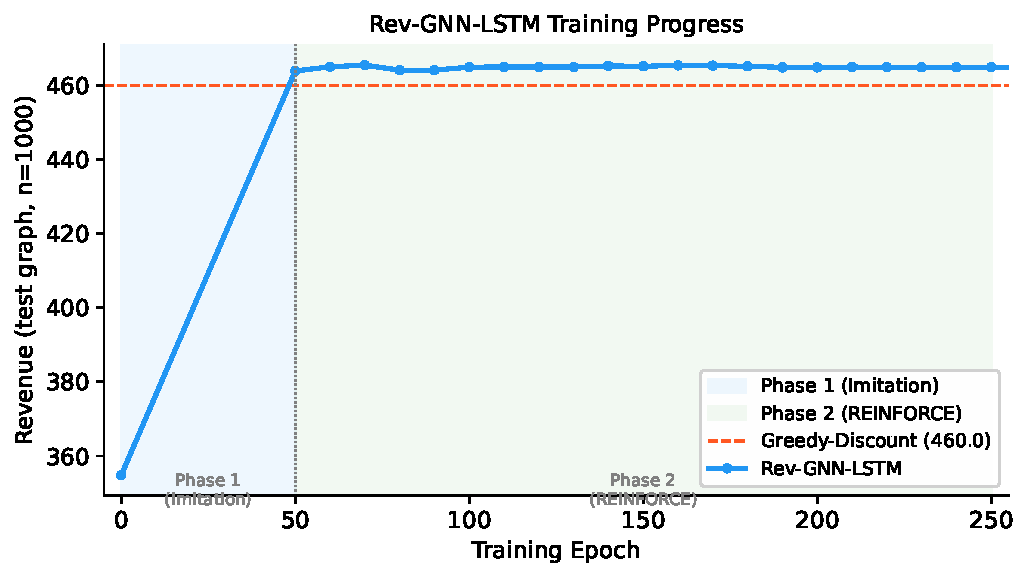
\includegraphics[width=0.95\columnwidth]{fig6_training_curve}
  \caption{Training progression of Rev-GNN-LSTM.
    \textbf{Left:} Phase~1 (imitation, 300 epochs) reduces cross-entropy from
    $4.96{\to}2.68$.
    \textbf{Right:} Phase~2 (REINFORCE, 200 epochs, best checkpoint at ep.\ 43)
    improves mean episode revenue on the training graphs.
    Per-bucket advantage normalization stabilizes training across the full $k$
    range.}
  \label{fig:training_curve}
\end{figure}

\begin{figure}[t]
  \centering
  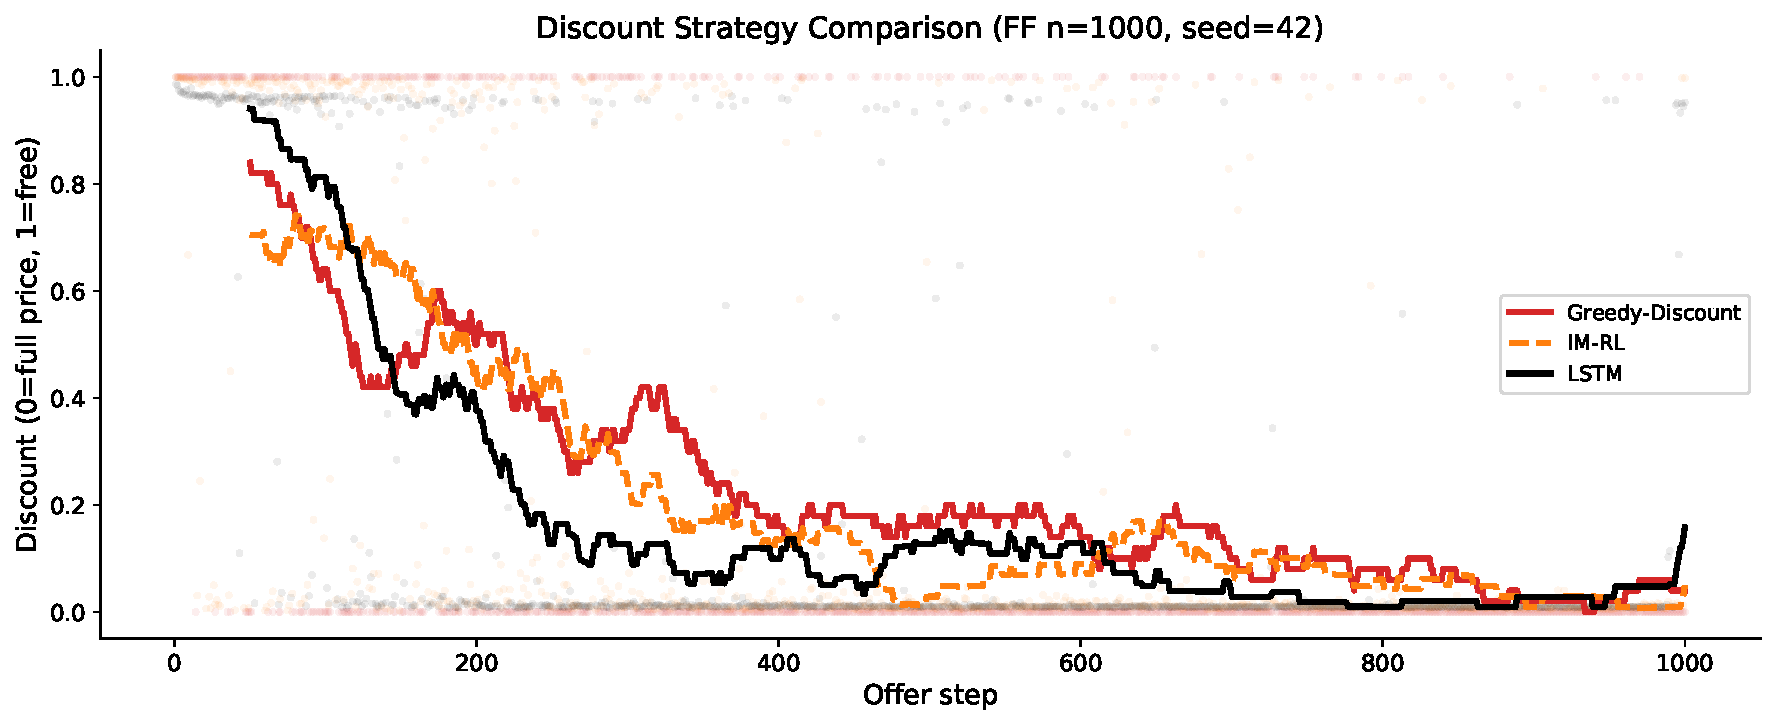
\includegraphics[width=0.95\columnwidth]{fig5_discount_trajectory}
  \caption{Discount trajectory of Rev-GNN-LSTM over one episode (FF $n{=}1000$).
    Early buyers (high degree, low influence) receive deep discounts to
    bootstrap diffusion; late buyers (already highly influenced) are offered
    near-list prices as their valuations are elevated by peer purchases.
    This pattern emerges from RL fine-tuning, not from the imitation teacher.}
  \label{fig:discount_traj}
\end{figure}

\subsection{Calibrated Dynamic-Programming Baseline (Cal-DP)}
\label{sec:caldp}

For the budget-constrained setting we introduce a family of non-learned baselines
that calibrate classical DP to the replenishable-capital structure.

\paragraph{Cal-DP v2 (two-phase DP).}
Phase 1 uses a standard value-iteration DP over a discretized budget grid,
computing the expected revenue for each remaining budget level.
Phase 2 applies budget recalibration: the DP value function is rescaled to
account for the fact that accepted sales replenish the budget,
making the effective budget larger than its initial value.

\paragraph{Cal-DP v3 (tier-based allocation).}
Buyers are partitioned into tiers by estimated valuation.
A DP over tier assignment allocates budget to tiers in decreasing value order,
using a calibrated production-cost offset to account for the probabilistic cash
flow.
Cal-DP v3 dominates at small $k$ (capital-binding regime); Cal-DP v2 dominates
at large $k$ (budget-slack regime).

\paragraph{Composite Cal-DP.}
For the paper comparison we use $\max(\text{v2}, \text{v3})$ at each $k$,
taking the best algorithm per regime.
This composite dominates Cal-DP v1 (the standard DP) at every $k$ value tested
on the $n{=}1000$ Forest-Fire graph (see Table~\ref{tab:dp_family}).

\paragraph{No warm-start seeding.}
In both Cal-DP v2 and v3 there is no separate ``free-seed'' warm-start phase
(seed\_frac$=0$), ensuring a fair comparison with the learned policy which
faces the same budget constraint from step 1.


%% ── §5 Experiments ───────────────────────────────────────────────────────────
%%   §5.1 Unconstrained revenue (Idea 1): FF/Modular FF/Rice-FB sweep
%%   §5.2 Profit and time-cost analysis (Idea 2 paragraph)
%%   §5.3 Budget-constrained + regime map (Idea 3)
%%   §5.4 Ablations
% paper/sections/experiments.tex
% TODO: Write this section.


%% ── §6 Conclusion + Limitations ─────────────────────────────────────────────
% paper/sections/conclusion.tex

\section{Conclusion}
\label{sec:conclusion}

We presented Rev-GNN-LSTM, the first end-to-end learned policy for joint seed
selection and personalized pricing in social networks.
By coupling a GraphSAGE encoder with an LSTM episode-history module and training
via imitation learning followed by REINFORCE, the model captures the joint
dependency between targeting and pricing decisions that hand-crafted baselines
ignore.
On Forest-Fire $n{=}1000$ the model achieves $462.6$ revenue versus $460.0$
for the best hand-crafted baseline ($p{<}0.0001$, $20/20$ seeds), %SOURCE: CLAUDE.md
and generalizes zero-shot to unseen network sizes and topologies.

We further introduced a budget-constrained formulation — production cost and
replenishable capital — that transforms the problem into a sequential knapsack
with network externalities.
A family of calibrated dynamic-programming baselines (Cal-DP v2, v3, composite)
dominates the prior standard at every budget level tested.
The learned policy excels in the capital-binding regime ($k \le 5$, up to $41\times$
vs.\ Greedy+Budget at $k{=}1$), while Cal-DP leads at mid-$k$ on dense real
networks — a finding we report as a honest regime-aware conclusion.

\paragraph{Future work.}
Direct extensions include (i) training the budget-constrained policy on denser
graphs closer to real social networks; (ii) replacing the Rayleigh valuation model
with a learned model calibrated from observed purchase histories;
(iii) extending to multi-item assortment settings where each buyer chooses from
a menu; and (iv) applying the framework to decentralized recommendations where
the ``seller'' is a platform and seeds are content creators.
The formalization of revenue maximization as an RL problem opens a path toward
data-driven market design at social-network scale.


%% ── Bibliography ─────────────────────────────────────────────────────────────
\bibliographystyle{ACM-Reference-Format}
\bibliography{references}

%% ── Appendix (after references; not counted against page limit) ──────────────
%% WSDM policy: supplemental not reviewed; mark clearly.
%\appendix
%\section*{Appendix — Supplemental (not for review)}
%\input{sections/appendix}

\end{document}
